% ============================================================
% CHAPTER 1 — GENERAL CONTEXT
% ============================================================
\chapter{General Context}
\chaptersommaire
\clearpage

\section*{Introduction}
This chapter lays the foundation of the project by presenting the host organization, the global and local market context, the challenges faced, and the objectives pursued. It also includes a comparative study of existing solutions, highlighting their limitations, before introducing the proposed solution.

\section{Presentation of the Host Organization}

Inherited Games Studio is a game development company specializing in the creation of educational and entertaining games. By leveraging immersive technologies such as virtual reality (VR) and augmented reality (AR), the studio enhances user engagement and learning experiences. Additionally, the integration of artificial intelligence (AI) allows for the personalization of content, ensuring dynamic and interactive gameplay.

\subsubsection*{A. Mission}

The mission of Inherited Games Studio is to develop innovative and immersive games that blend education and entertainment. Through the use of cutting-edge technology, the company aims to offer users enriching, interactive, and engaging experiences that enhance learning while maintaining a high level of fun.

\begin{figure}[H]
\centering

\includegraphics[height=3cm, keepaspectratio]{images/igs_logo.png}
\caption{Inherited Games Studio Logo}
\end{figure}

\subsubsection*{B. Methodology}

To achieve its objectives, Inherited Games Studio follows a structured development approach that includes:

\begin{itemize}
  \item \textbf{Immersive Technologies:} Using VR and AR to create realistic and engaging environments.
  \item \textbf{AI-Driven Personalization:} Adapting gameplay and learning paths based on user interactions to enhance engagement and retention.
  \item \textbf{Multiplayer and Gamification:} Encourage social interaction and competition through multiplayer experiences and game-based incentives.
  \item \textbf{Continuous Optimization:} Analyze user feedback and performance metrics to refine and improve game mechanics.
  \item \textbf{Educational and Entertaining Design:} Ensure a balance between learning and enjoyment to maximize the impact of each game. By combining technology, creativity, and user-centered design, Inherited Games Studio continues to push the boundaries of immersive and interactive learning experiences.
\end{itemize}


\section{Project Presentation}
\subsection{Project Context}
The project was carried out at \textbf{Inherited Games Studio (IGS)}, a Tunisian game development company specializing in educational and entertaining games. By leveraging immersive technologies such as \textbf{Virtual Reality (VR)} and \textbf{Augmented Reality (AR)}, combined with \textbf{Artificial Intelligence (AI)} for personalization, IGS aims to deliver interactive and engaging experiences.

\subsection{Global Market Context}
The global digital content economy is experiencing remarkable expansion. The worldwide \textbf{3D model marketplace} was valued at \textbf{USD 1.92 billion in 2023} and is projected to reach \textbf{USD 4.86 billion by 2031}, growing at a \textbf{CAGR of 11.2\%}. Demand is driven primarily by:
\begin{itemize}
    \item Video games (38.2\% of consumption),
    \item Architectural visualization (22.1\%),
    \item Film \& television production (17.8\%).
\end{itemize}

\subsection{The Tunisian Gap}
Despite this global growth, Tunisia lacked a dedicated 3D digital asset marketplace before this project. Local developers and studios depended on foreign platforms such as Unity Asset Store, Sketchfab, Fab, and CGTrader, which imposed:
\begin{itemize}
    \item Dollar-denominated pricing,
    \item Foreign payment gateways,
    \item Policies misaligned with the local creative economy.
\end{itemize}

IGS identified this gap and commissioned the development of \textbf{IGS Marketplace}, the first Tunisian platform for 3D asset exchange, designed to serve both internal workflows and external communities.


\subsection{Objectives}
IGS faced several operational challenges that were transformed into clear project objectives:
\begin{itemize}
    \item \textbf{Centralized Asset Repository}: Create a unified catalog with advanced search and categorization.
    \item \textbf{Monetization Platform}: Enable external sales of surplus assets with secure payment integration.
    \item \textbf{Role-Based Access Control (RBAC)}: Implement six hierarchical roles to ensure secure and differentiated access.
    \item \textbf{Unified Collaboration Tools}: Provide integrated project management, notifications, and real-time communication.
    \item \textbf{Local Adaptation}: Offer Tunisian payment methods (Flouci) alongside Stripe, ensuring accessibility for local creators.
    \item \textbf{Intern Management}: Introduce supervised workflows and limited access for interns.
\end{itemize}
\section{Comparative Study of Existing Solutions}

\subsection{Analysis}
The international landscape is dominated by four major platforms. Each offers unique strengths but fails to meet IGS’s combined requirements of self-hosting, RBAC, internal workflows, and AI integration.

\subsubsection{Unity Asset Store}
Launched in 2010, Unity Asset Store is tightly integrated with the Unity Editor, offering millions of assets. However, it is engine-specific, lacks RBAC, and provides no internal team tools.

\begin{figure}[h]
\centering
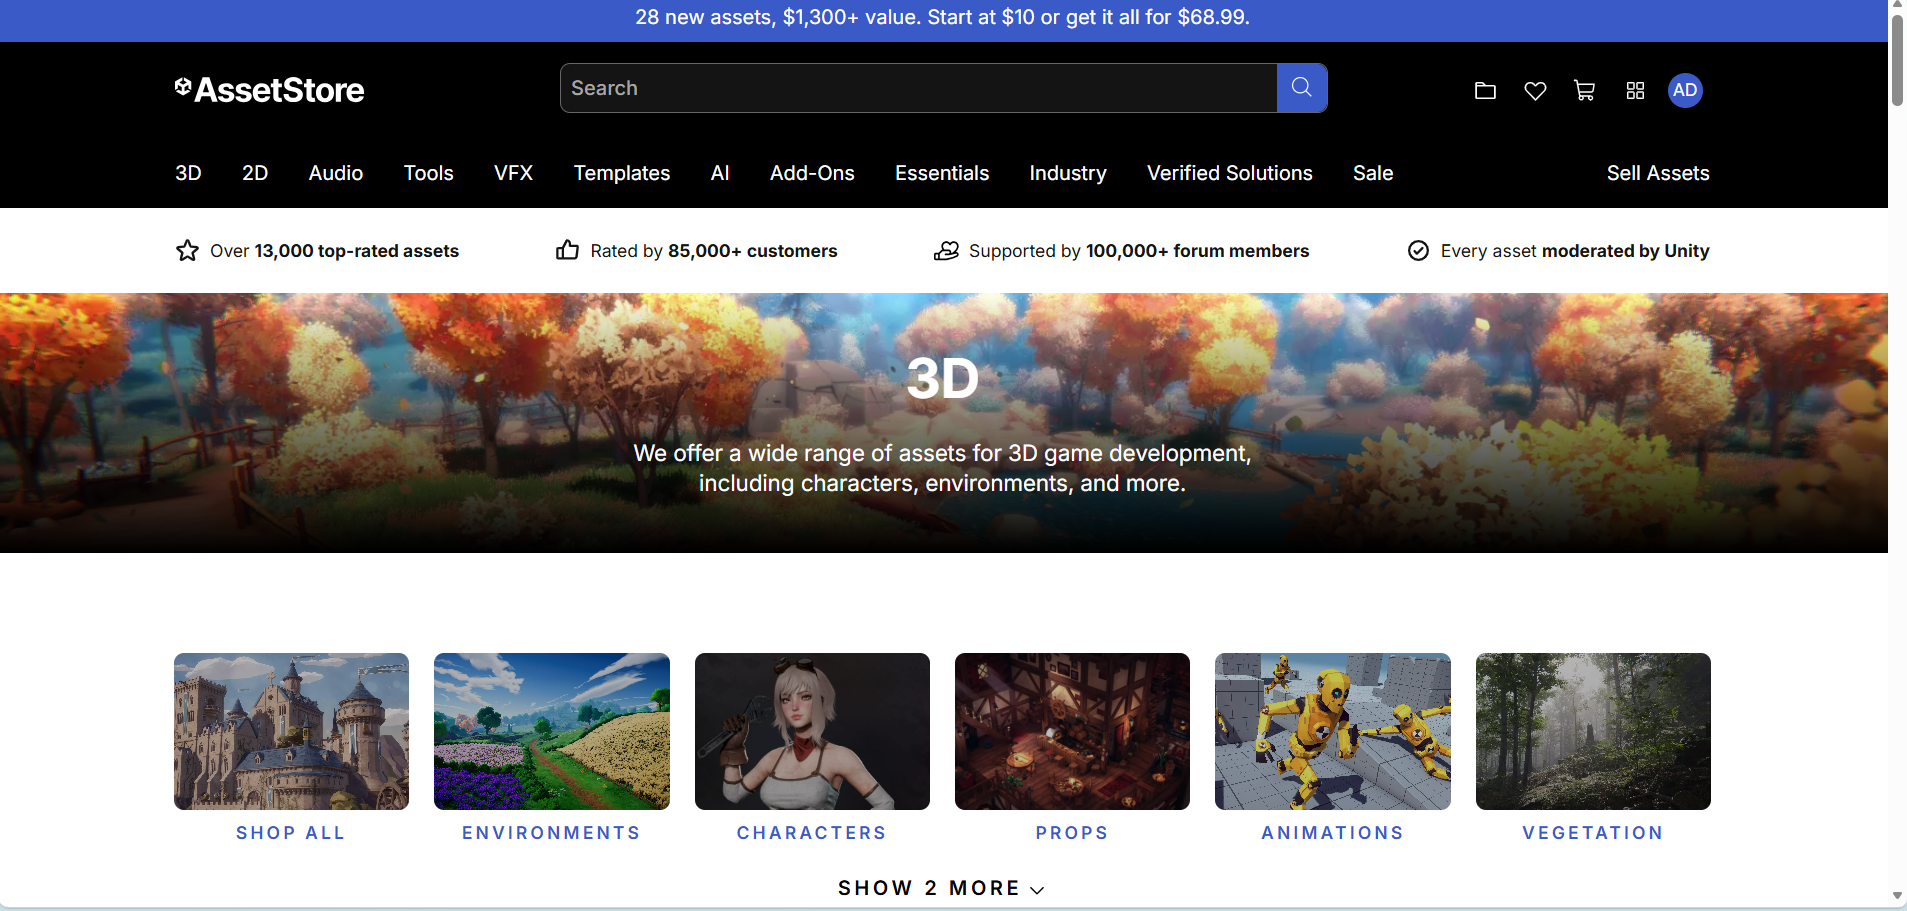
\includegraphics[width=0.5\textwidth]{images/existant/unity.png}
\caption{Unity Asset Store}
\end{figure}

\subsubsection{Fab (Epic Games)}
Fab, Epic Games’ unified marketplace, supports multiple engines and benefits from Unreal Engine integration. Despite its breadth, it lacks customization, internal workflows, and AI-powered features.

\begin{figure}[h]
\centering
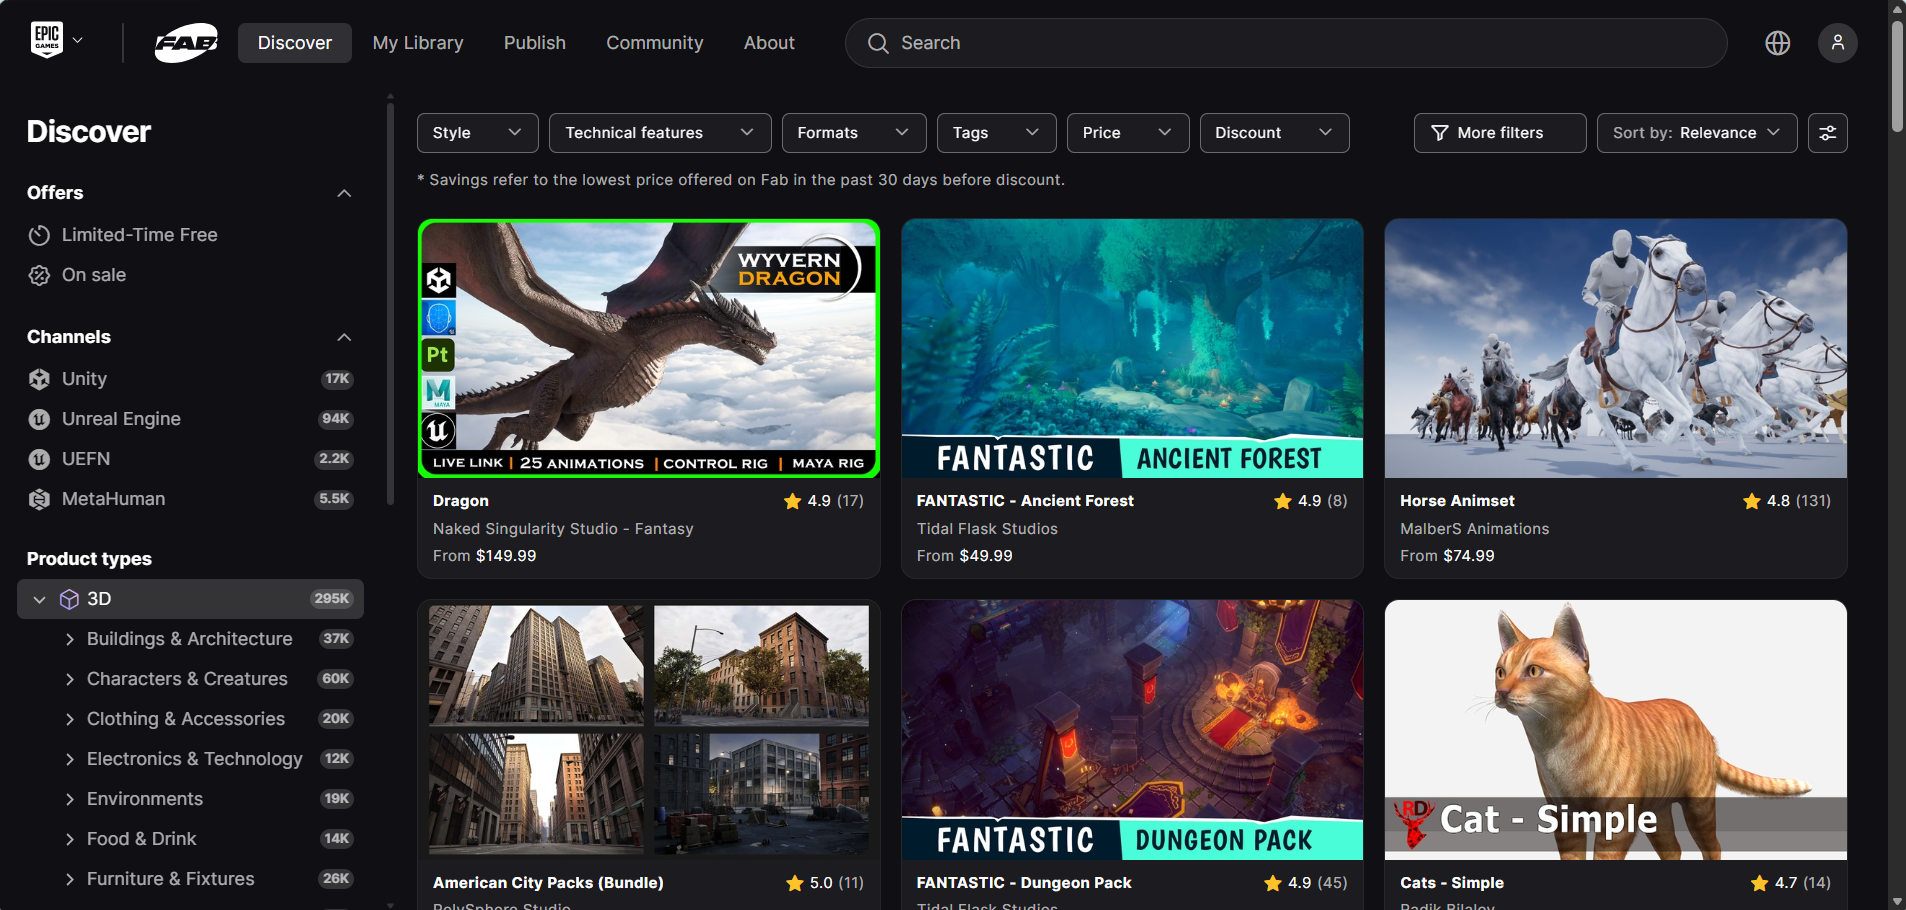
\includegraphics[width=0.5\textwidth]{images/existant/fab.png}
\caption{Fab Marketplace}
\end{figure}

\subsubsection{Sketchfab}
Sketchfab excels in in-browser 3D visualization and supports multiple formats. It is widely used for showcasing models but does not provide monetization flexibility, RBAC, or internal studio management.

\begin{figure}[h]
\centering
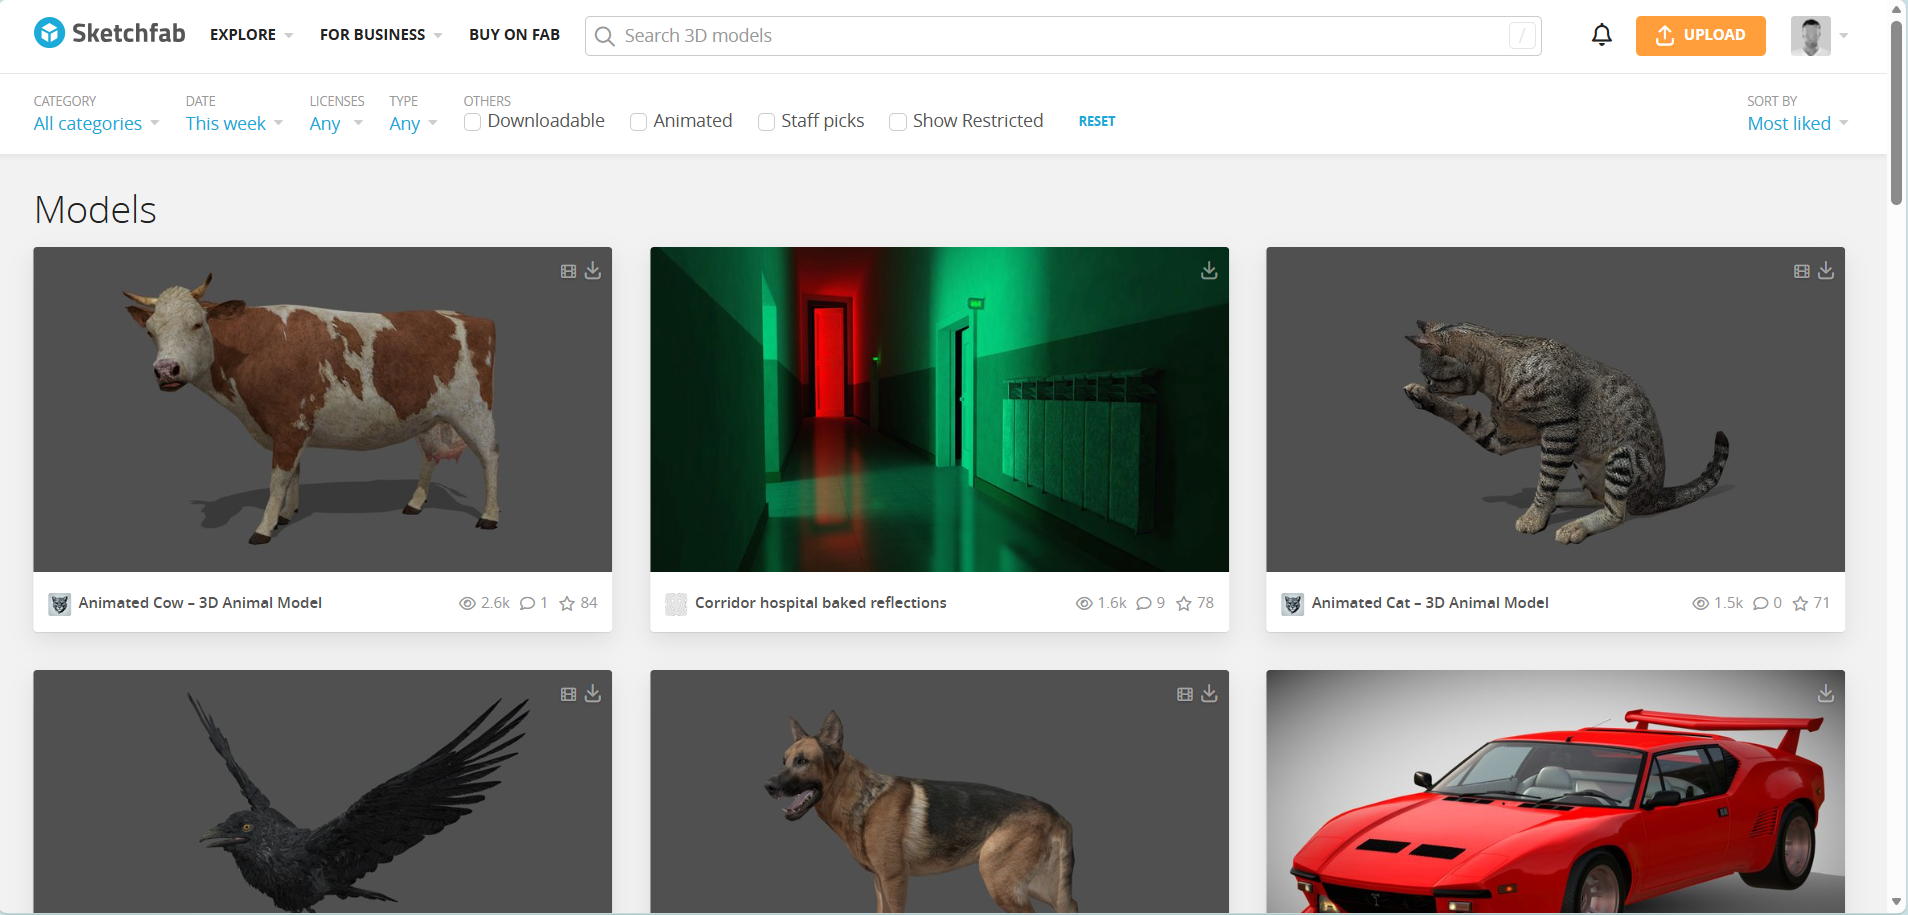
\includegraphics[width=0.5\textwidth]{images/existant/sketchfab.png}
\caption{Sketchfab Platform}
\end{figure}

\subsubsection{CGTrader}
CGTrader offers a large catalog and supports multiple engines. However, it is externally hosted, lacks internal collaboration tools, and does not integrate AI or role-based workflows.

\begin{figure}[h]
\centering
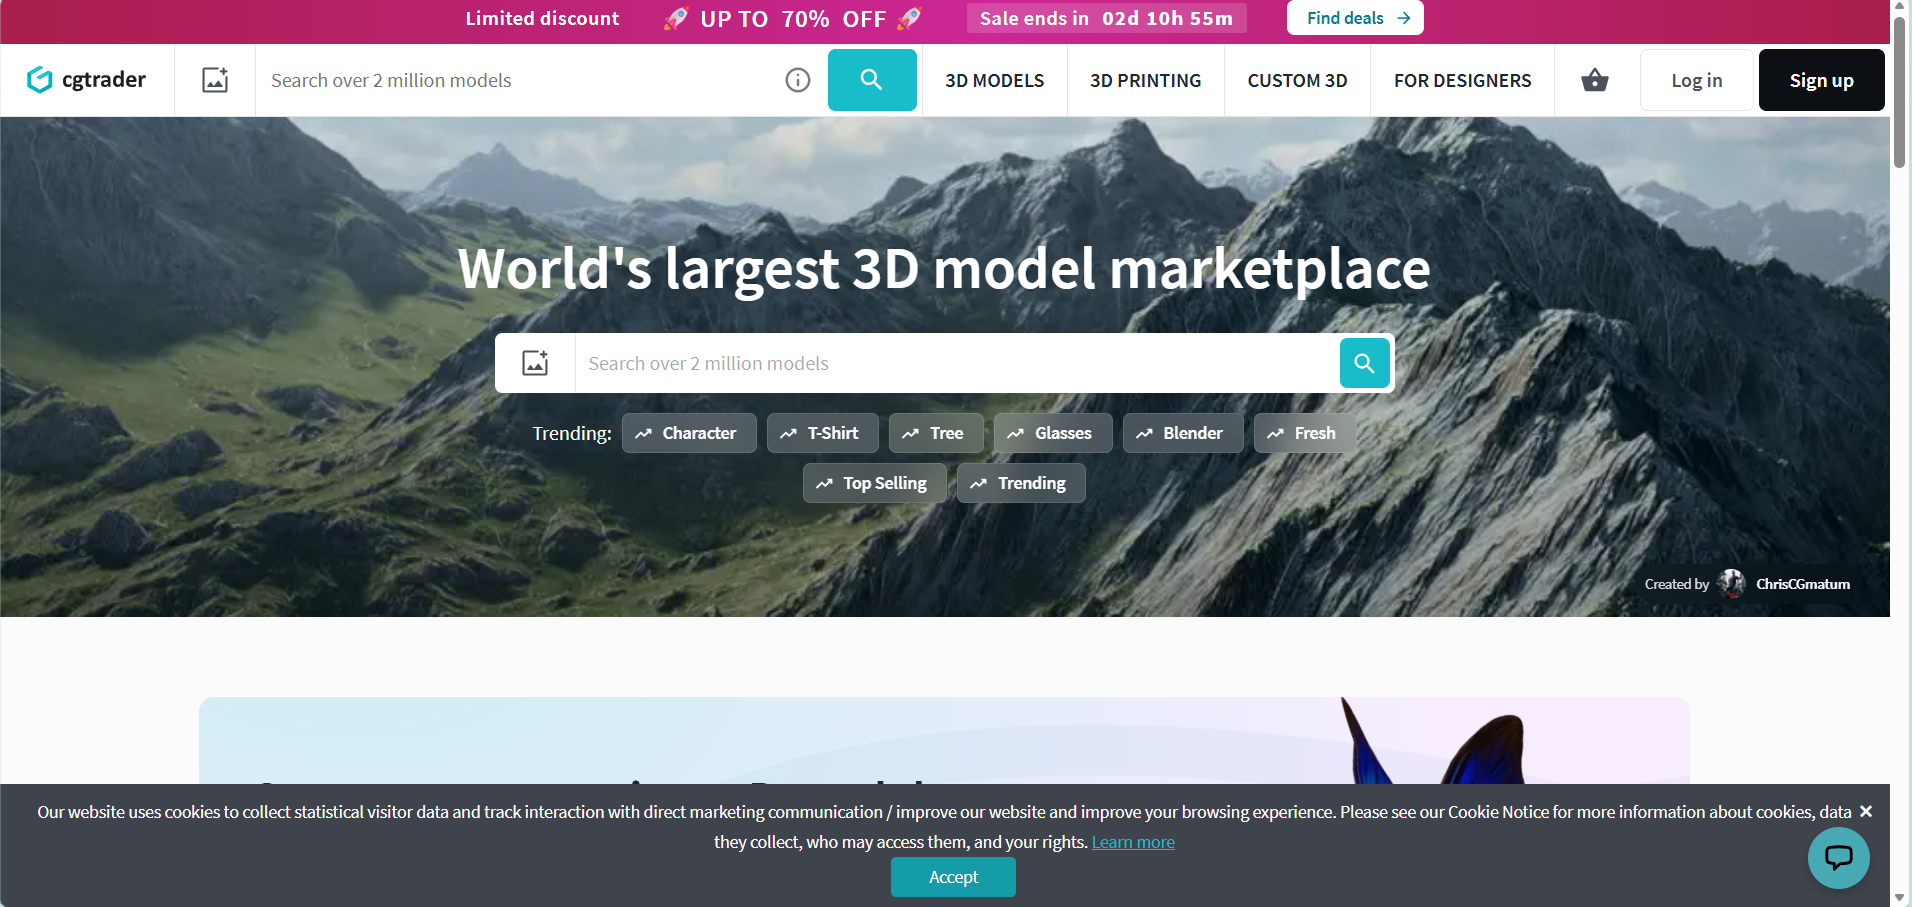
\includegraphics[width=0.5\textwidth]{images/existant/cgtrader.png}
\caption{CGTrader Marketplace}
\end{figure} 

\subsection{Critics}
\begin{itemize}
    \item \textbf{Unity Asset Store}: Limited to Unity, no RBAC, no internal workflows.
    \item \textbf{Fab}: Strong Unreal integration but lacks customization and AI.
    \item \textbf{Sketchfab}: Excellent visualization but weak in monetization and team features.
    \item \textbf{CGTrader}: Large catalog but externally controlled, no studio-oriented tools.
\end{itemize}

None of these platforms combine marketplace features, internal ERP-style modules, RBAC, and AI services in a single self-hosted solution.

\section{Proposed Solution}
The proposed solution is a \textbf{full-stack web platform} composed of two interconnected applications:

\begin{enumerate}
    \item \textbf{IGS Marketplace}: Public-facing marketplace for asset listing, purchase, and moderation. Features include a 3D interactive viewer, Stripe \& Flouci checkout, subscription system, and an AI chatbot assistant.
    \item \textbf{IGS Workspace}: Internal dashboard for employees and interns. Features include task management, project ERP modules, analytics, and real-time chat.
\end{enumerate}

Both applications share the same backend API (Express.js), PostgreSQL database, and JWT authentication, enabling seamless Single Sign-On (SSO).

\subsection{Development Methodology: Scrum}

\textbf{Scrum} was selected as the development methodology because requirements emerged progressively throughout the internship, the company supervisor (Mme. Nour Ltaief) naturally assumes the Product Owner role, the academic supervisor (Mr. Sami Ben Amor) assumes the Scrum Master role, and sprint reviews align with mandatory internship progress meetings.

The project was divided into \textbf{eight sprints}, each lasting approximately two to three weeks:

\begin{table}[H]
\centering
\caption{Sprint Planning Overview}
\begin{tabular}{C{1.2cm} L{4.5cm} L{7.8cm}}
\toprule
\textbf{Sprint} & \textbf{Theme} & \textbf{Key Deliverables} \\
\midrule
0 & Research \& Architecture       & Architecture design, DB schema, environment setup \\
1 & Core Infrastructure            & Backend, PostgreSQL, JWT auth, RBAC (6 roles) \\
2 & Asset Marketplace Core         & Catalog, 3D viewer, seller upload, cart, Stripe \\
3 & Content \& Administration      & Reviews, notifications, admin panel, subscriptions \\
4 & Advanced Role Features         & Intern workflow, seller analytics, trading, groups \\
5 & IGS Workspace                  & Companion app, task management, real-time chat \\
6 & AI Integration                 & ML models, sentiment analysis, chatbot \\
7 \& 8 & AI Expansion \& Polish   & Recommendation engine, UI overhaul, admin dashboard \\
\bottomrule
\end{tabular}
\end{table}

% ---- 1.6 TECHNOLOGY STACK ----
\section{Technology Stack}

\begin{table}[H]
\centering
\caption{Technology Stack Summary}
\begin{tabular}{L{3cm} L{4.5cm} L{6cm}}
\toprule
\textbf{Layer} & \textbf{Technology} & \textbf{Role / Justification} \\
\midrule
\multirow{3}{*}{Frontend}
  & React 18 + Vite           & SPA framework — fast HMR, component model \\
  & Three.js / Model Viewer   & 3D asset viewer in the browser \\
  & TailwindCSS               & Utility-first responsive styling \\
\midrule
\multirow{3}{*}{Backend}
  & Node.js + Express.js      & REST API — non-blocking, JSON-native \\
  & Socket.io                 & WebSocket real-time events (chat, notifications) \\
  & HuggingFace / Mistral-7B  & AI review analysis, chatbot, recommendations \\
\midrule
\multirow{3}{*}{Data \& Auth}
  & PostgreSQL 16             & Primary relational database \\
  & Supabase                  & Scalable file hosting for 3D assets \\
  & Supabase Auth             & Authentication, sessions, and JWT-based access \\
\midrule
Payments & Stripe             & Secure card payment processing \\
\midrule
\multirow{2}{*}{Dev Tools}
  & Git + GitHub              & Version control and CI/CD \\
  & Postman + draw.io         & API testing and UML diagram preparation \\
 
\bottomrule
\end{tabular}
\end{table}

% ---- 1.7 WORK ENVIRONMENT ----
\section{Work Environment}

The project was developed in a modern full-stack environment combining frontend, backend,
database, storage, payment, AI, version-control, and documentation tools. The following
overview summarizes the main tools used during the internship.

\newcommand{\toollogo}[2]{%
\begin{minipage}{0.15\textwidth}
\centering
\includegraphics[height=0.72cm, keepaspectratio]{images/#1}\\[-1pt]
{\scriptsize #2}
\end{minipage}
}

\begin{table}[H]
\centering
\caption{Software Work Environment}
\renewcommand{\arraystretch}{1.35}
\begin{tabularx}{\textwidth}{L{3cm} X}
\toprule
\textbf{Category} & \textbf{Tools} \\
\midrule
Frontend &
\toollogo{logo_react.png}{React}
\toollogo{logo_vite.png}{Vite}
\toollogo{logo_threejs.png}{Three.js}
\toollogo{logo_tailwindcss.png}{TailwindCSS} \\
\midrule
Backend &
\toollogo{logo_nodejs.png}{Node.js}
\toollogo{logo_express.png}{Express.js}
\toollogo{logo_socketio.png}{Socket.io}
\toollogo{logo_jwt.png}{JWT} \\
\midrule
Data, Auth, Storage &
\toollogo{logo_postgresql.png}{PostgreSQL}
\toollogo{logo_supabase.png}{Supabase}
\toollogo{logo_supabase.png}{Supabase Auth}
\toollogo{logo_stripe.png}{Stripe} \\
\midrule
AI and Testing &
\toollogo{logo_huggingface.png}{HuggingFace}
\toollogo{logo_postman.png}{Postman}
\toollogo{logo_eslint.png}{ESLint}
\toollogo{logo_npm.png}{npm} \\
\midrule
DevOps and Documentation &
\toollogo{logo_github.png}{GitHub}
\toollogo{logo_githubactions.png}{Actions}
\toollogo{logo_docker.png}{Docker}
\toollogo{logo_drawio.png}{draw.io} \\
\midrule
Development IDE &
\toollogo{logo_git.png}{Git}
\toollogo{logo_latex.png}{XeLaTeX}
\toollogo{logo_postman.png}{API Tests}
\toollogo{logo_drawio.png}{UML} \\
\bottomrule
\end{tabularx}
\end{table}

\section*{Conclusion}
This chapter established the project context: the host organization IGS and its operational challenges, the comparative analysis confirming the absence of a dedicated 3D marketplace in Tunisia, the proposed two-application solution, the Scrum methodology applied across eight sprints, the technology stack, and the work environment. The following chapter details the functional and non-functional requirements of the system.
